\documentclass{ci5652}
\usepackage{graphicx,amssymb,amsmath}
\usepackage[utf8]{inputenc}
\usepackage[spanish]{babel}
\usepackage{hyperref}
\usepackage{subfigure}
\usepackage{paralist}
\usepackage[ruled,vlined,linesnumbered]{algorithm2e}

%----------------------- Macros and Definitions --------------------------

% Add all additional macros here, do NOT include any additional files.

% The environments theorem (Theorem), invar (Invariant), lemma (Lemma),
% cor (Corollary), obs (Observation), conj (Conjecture), and prop
% (Proposition) are already defined in the ci5652.cls file.

\graphicspath{ {plots/} }

%----------------------- Title -------------------------------------------

\title{Problema de selección de prototipo (IS/PS):\\ 
       Un enfoque con metaheurísticas}

\author{Juan Carlos Arocha Ovalles
        \and
        Matteo José Ferrando Briceño}

%------------------------------ Text -------------------------------------

\begin{document}
\thispagestyle{empty}
\maketitle


\begin{abstract}
El uso de clasificadores para determinar la clase de algún \textit{documento} está intimamente relacionado con el conjuntos de datos \textit{TR} con el que son entrenados. Un TR que represente adecuadamente a la muestra contiene potencialmente una gran cantidad de instancias, lo que genera un entrenamiento y una clasificación lenta. El objetivo de este estudio es encontrar un subconjunto de TR considerablemente más pequeño y con la misma capacidad de entrenamiento, es decir, que un clasificador que entrene con dicho subconjunto arroje los mismos resultado que entrenando con el TR original.


\end{abstract}

\section{Problema de selección de prototipo}

En el campo de clasificación de documentos, la calidad de clasificadores como \textit{K-NN} depende del TR con el cual sean entrenados. Un problema que se encuentra a la hora de elegir el TR es la selección de las intancias que lo conforman. Una gran cantidad instancias que representen las diferentes clases, pueden llevar a una buena clasificación, pero a su vez llevan a un entrenamiento y a un desempeño lento por parte de los clasificadores.

Es por ello que se ha intentado reducir este conjunto para disminuir el tiempo de entrenamiento y clasificación, pero manteniendo la calidad de los resultados que se obtengan.

Este problema es bastante común en diversas áreas de ciencias de la computación, por ejemplo, procesamiento y etiquetado de imágenes, análisis de \textit{big data}, análisis de lenguaje natural, \textit{Data Mining}, entre otros por lo que ha sido bastante estudiado y existen diversas soluciones propuestas.

\section{Trabajos anteriores}
\label{sect:works}

Entre las soluciones que se estudiaron en el estado del arte, en~\cite{pgnn2002} Toussaint describe soluciones de tipo \textit{Greedy} como CNN, RNN y MCNN, las cuales demuestran una baja complejidad de tiempo y cuyos resultados son aceptables pero no optimales.Cano y Herrera en ~\cite{evo2003}, proponen utiliazr algoritmos evolutivos solucionar el problema de selección de instancias para extracción de conocimientos en bases de datos (KDD), presentan una función de evaluación de calidad que se utilizaron para las pruebas; finalmente, concluyen que para KDD, los algoritmos evolutivos mejoran tanto la reducción del subconjunto, como la presición. Luego García y Derrac, con apoyo de Cano y Herrera, en ~\cite{psfnn2012} hacen un análisis extenso de los diversos algritmos basados en el algoritmo \textit{K-NN}. 

\section{Metaheurísticas}
\label{sect:meta}

Como se vió en~\cite{evo2003}, una forma de resolver el problema IS/PS es usando metaheurísticas. Una metaheurística es un método genérico de solución de problemas computacionales, que no toma en cuenta el enunciado del problema sino la representación de sus soluciones, para luego mejorarlas en un tiempo eficiente pero que no asegura la optimalidad.

La mayoría de las metaheurísticas parten de una solución inicial, y a través de métodos iterativos, mejoran dicha solución, manteniendo la mejor de todas vista hasta el momento. La condición de parada de las mismas suelen variar entre un límite de tiempo, de iteraciones o que el espacio de búsqueda no provea mejores soluciones.

Para poder realizar pruebas usando metaheurísticas, se necesita una representación de la solución del problema planteado. En este caso, IS/PS fue representado con dos conjuntos: \textbf{SP} que corresponde a las instancias que se encuentran dentro del subconjunto de TR seleccionado y \textbf{UP} que corresponde al resto de las instancias que no están en el mismo. Por otro lado, también es necesario tener una funcion que sea capaz de evaluar una solución y que de este modo dos soluciones sean comparables. Como se vió en la sección~\ref{sect:works}, la calidad del subconjunto de TR seleccionado depende de la calidad de clasificación y del tamaño del mismo. La calidad se puede representar como el porcentaje de documentos bien clasificados, y el tamaño como el porcentaje de reducción de TR, lo que genera una función con dos variables. Para los experimentos se propusieron tres funciones:

\begin{equation}\label{eq:weight}
f(cl,rd) = \alpha\times cl + (1 - \alpha)\times rd
\end{equation}

\begin{equation}\label{eq:sqr}
f(cl,rd) = cl^{2}\times rd^{2}
\end{equation}

\begin{equation}\label{eq:exp}
f(cl,rd) = \beta^{cl\times rd}
\end{equation}

Donde $cl$ corresponde al porcentaje de classificación correcta, $rd$ al porcentaje de reducción de TR, $\alpha$ al peso en porcentaje (entre 0 y 1) que tiene $cl$ con respecto a $rd$ y $\beta$ a un número real arbitrario. La razón por la cual de toman estas funciones es porque se busca penalizar la puntuación obtenida por las mismas cuando cualquier de los dos atributos, sea $cl$ o $rd$, tengan valores muy bajos.

Por otra parte, también es necesario definir un operador de vecindad, el cual consiste en una función capaz de generar nuevas soluciones a partir de cualquier solución. El mismo depende de la metaheurística aplicada a problema.

En los experimentos realizados en este estudio, se consideró el uso de búsqueda local, la cual consiste en partir de una solución inicial, que va a ser modificada por un operador de vecindad que genera otra solución factible. Luego, la solución actual se compara con la solución generada a través de una función de evaluación de calidad, y se desecha la peor de ambas para recurrir en el mismo proceso con la restante.


\section{Experimentos con búsqueda local}

Como fue descrito en la sección~\ref{sect:meta}, se tomó la representación de \textbf{SP}y \textbf{UP} para las soluciones y las funciones de evaluación se tomaron las funciones~\ref{eq:sqr}, ~\ref{eq:weight} y~\ref{eq:exp}, .

Para ~\ref{eq:exp}, $\beta$ tomó el valor de \textit{Euler} por la forma en que la función exponencial crece. Como se puede ver en la figura~\ref{fig:euler3}, la misma penaliza a los valores más bajos, pues su crecimiento en ese punto es lento y a medida que los valores suben, el valor de la función crece de forma más violenta. En las figuras~\ref{fig:squared3} y~\ref{fig:weighted3} se puede notar que~\ref{eq:sqr} y~\ref{eq:weight} tienen un comportamiento parecido a~\ref{eq:exp} pero menos pronunciado. 

El operador de vencidad que se definió, consiste en una función que intercambia $K$ instancias entre \textbf{SP} y \textbf{UP} para generar nuevas soluciones, donde $K$ es un parámetro a calibrar dependiendo del problema de clasificación.

\begin{algorithm}
 \DontPrintSemicolon
 \vspace*{0.1cm}
 \KwIn{SP, UP : Conjunto de puntos, K : Entero}
 \KwOut{SP', UP'}
 \ForEach{$1 \dots K$}{
  $sacar = booleano\_al\_azar()$\;
  \If{$sacar$}{
	$punto = punto\_al\_azar(SP)$\;
	$SP' = SP\ \backslash{}\ \{punto\}$\;
	$UP' = UP\ \cup\ \{punto\}$\;
  }
  \Else{
	$punto = punto\_al\_azar(UP)$\;
	$UP' = UP\ \backslash{}\ \{punto\}$\;
	$SP' = SP\ \cup\ \{punto\}$\;
  }
 }
 \vspace*{0.1cm}
 \caption{Operador de vecindad}
\end{algorithm}

\begin{figure}[p]
	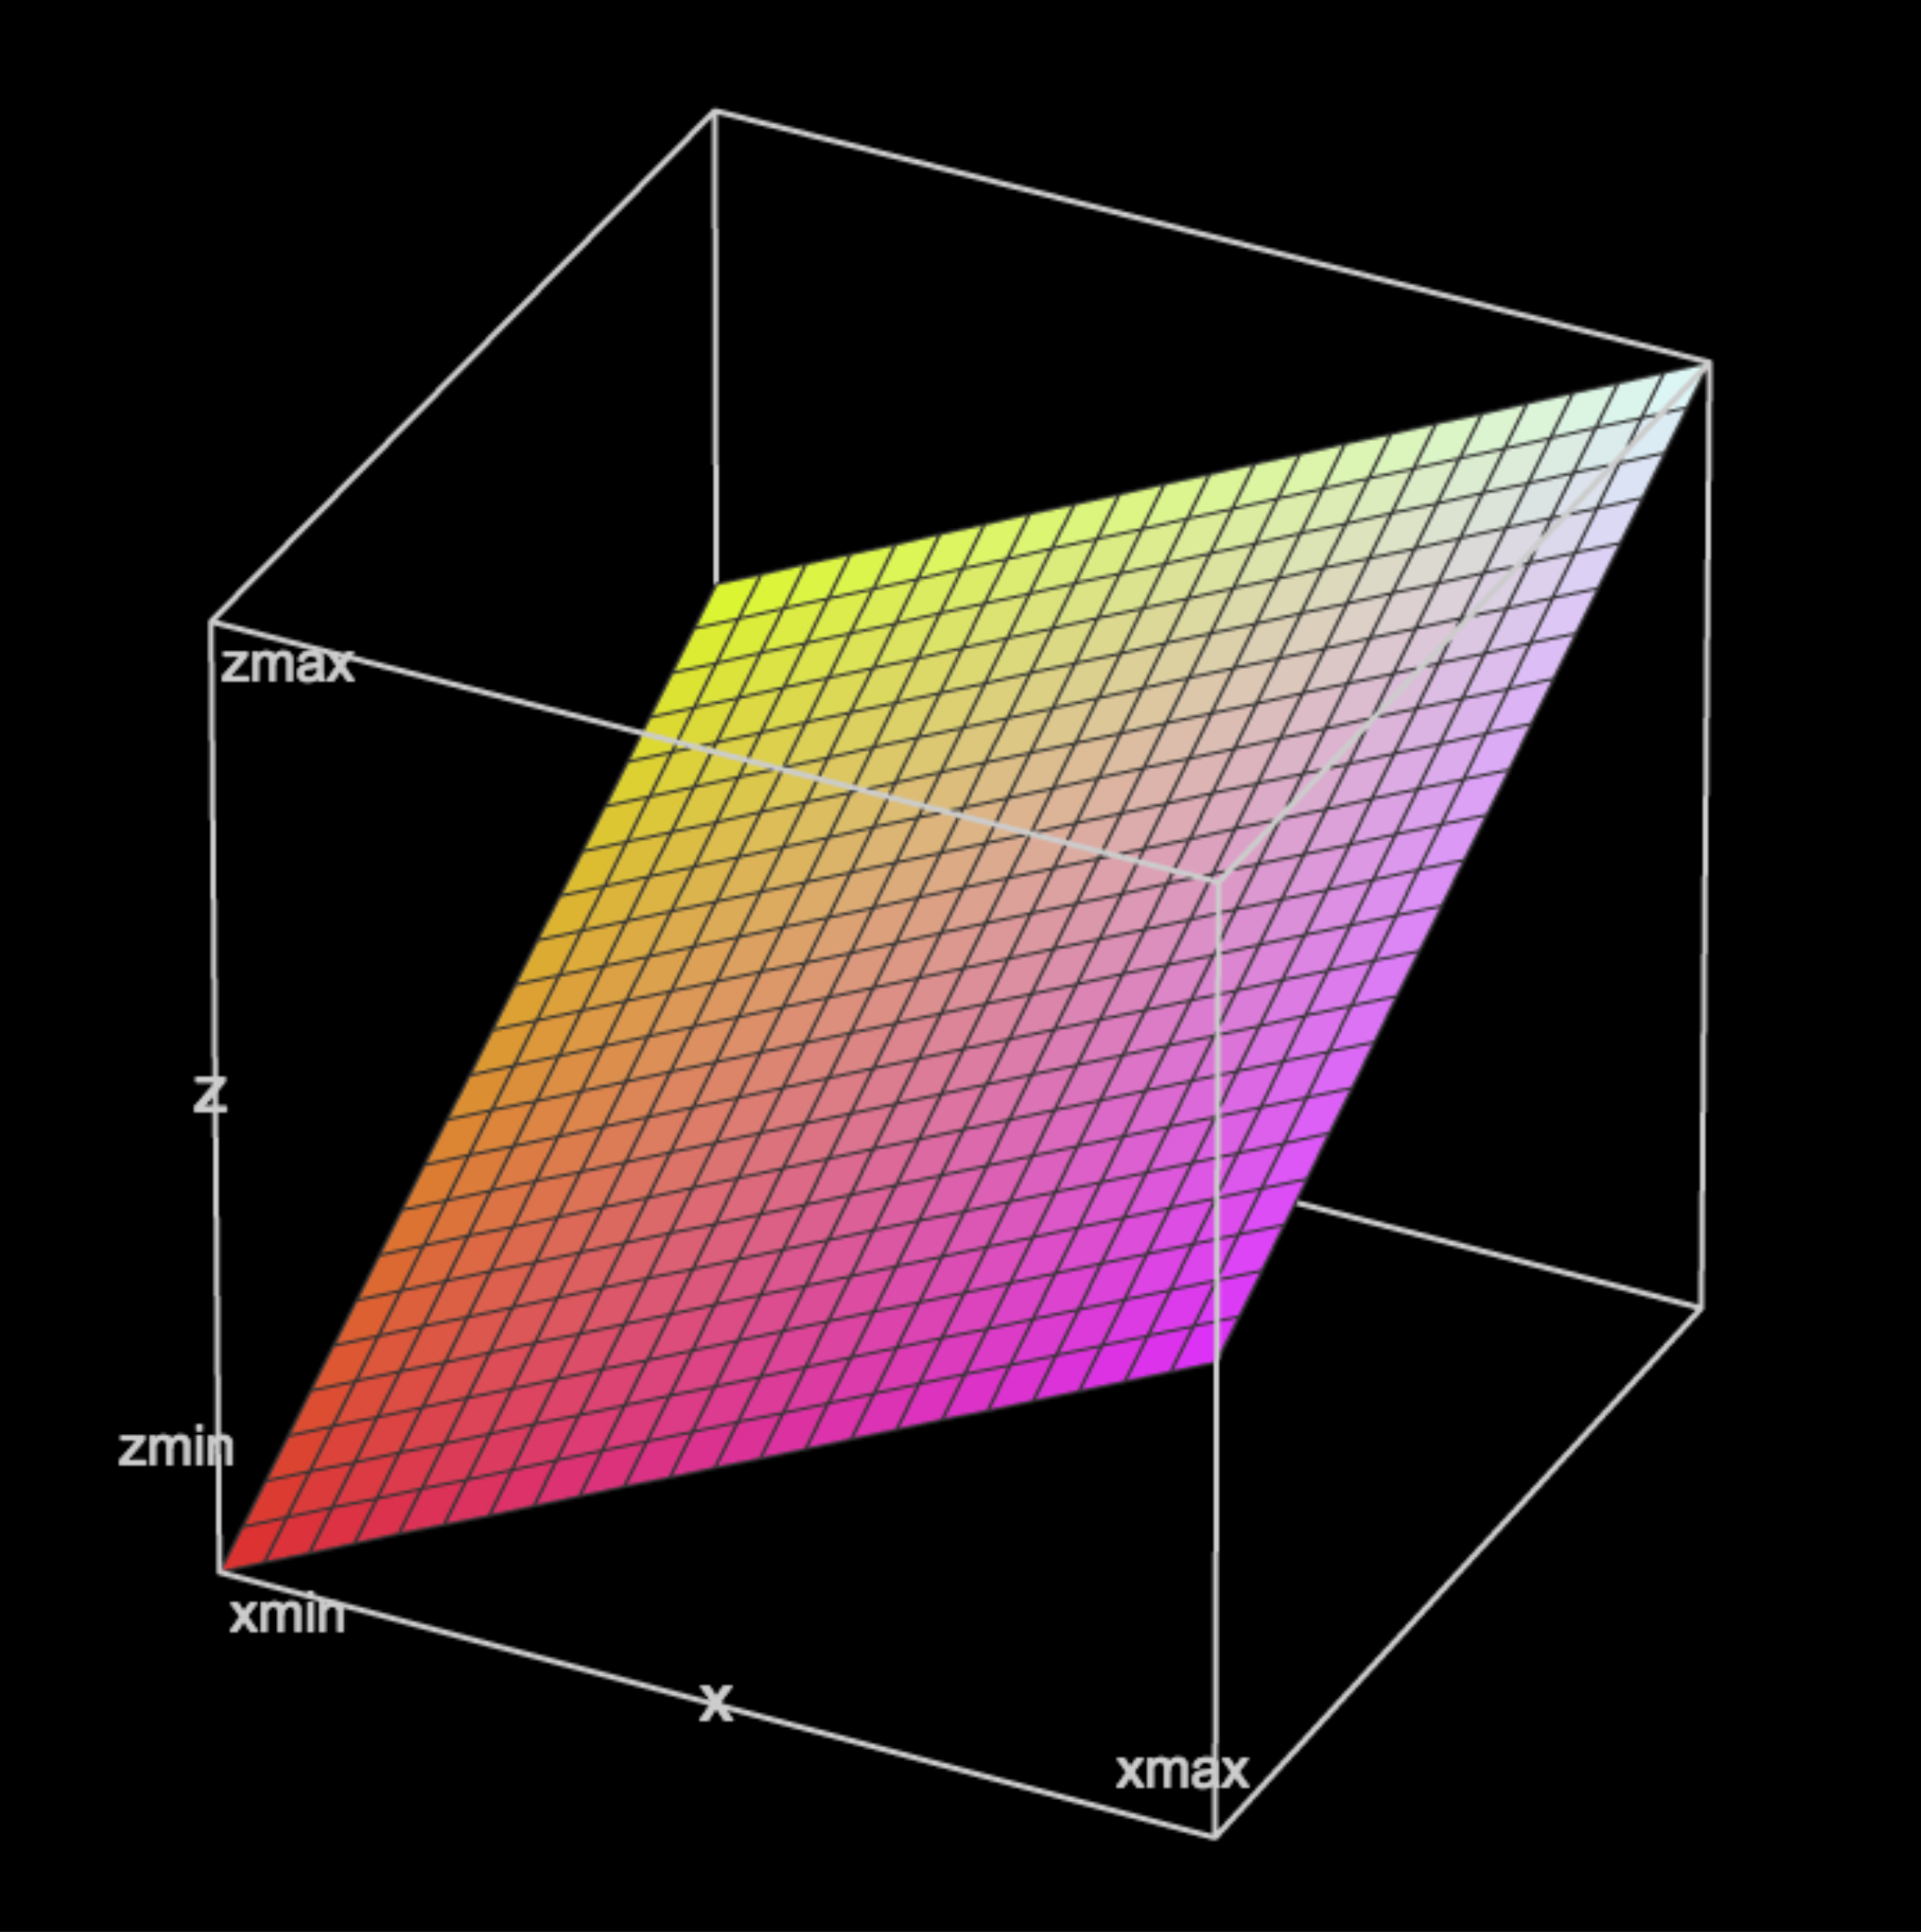
\includegraphics[width=\linewidth]{weighted-3b}
	\caption{Pesada, ecuación~\ref{eq:weight}}
	\label{fig:weighted3}
\end{figure}

\begin{figure}[p]
	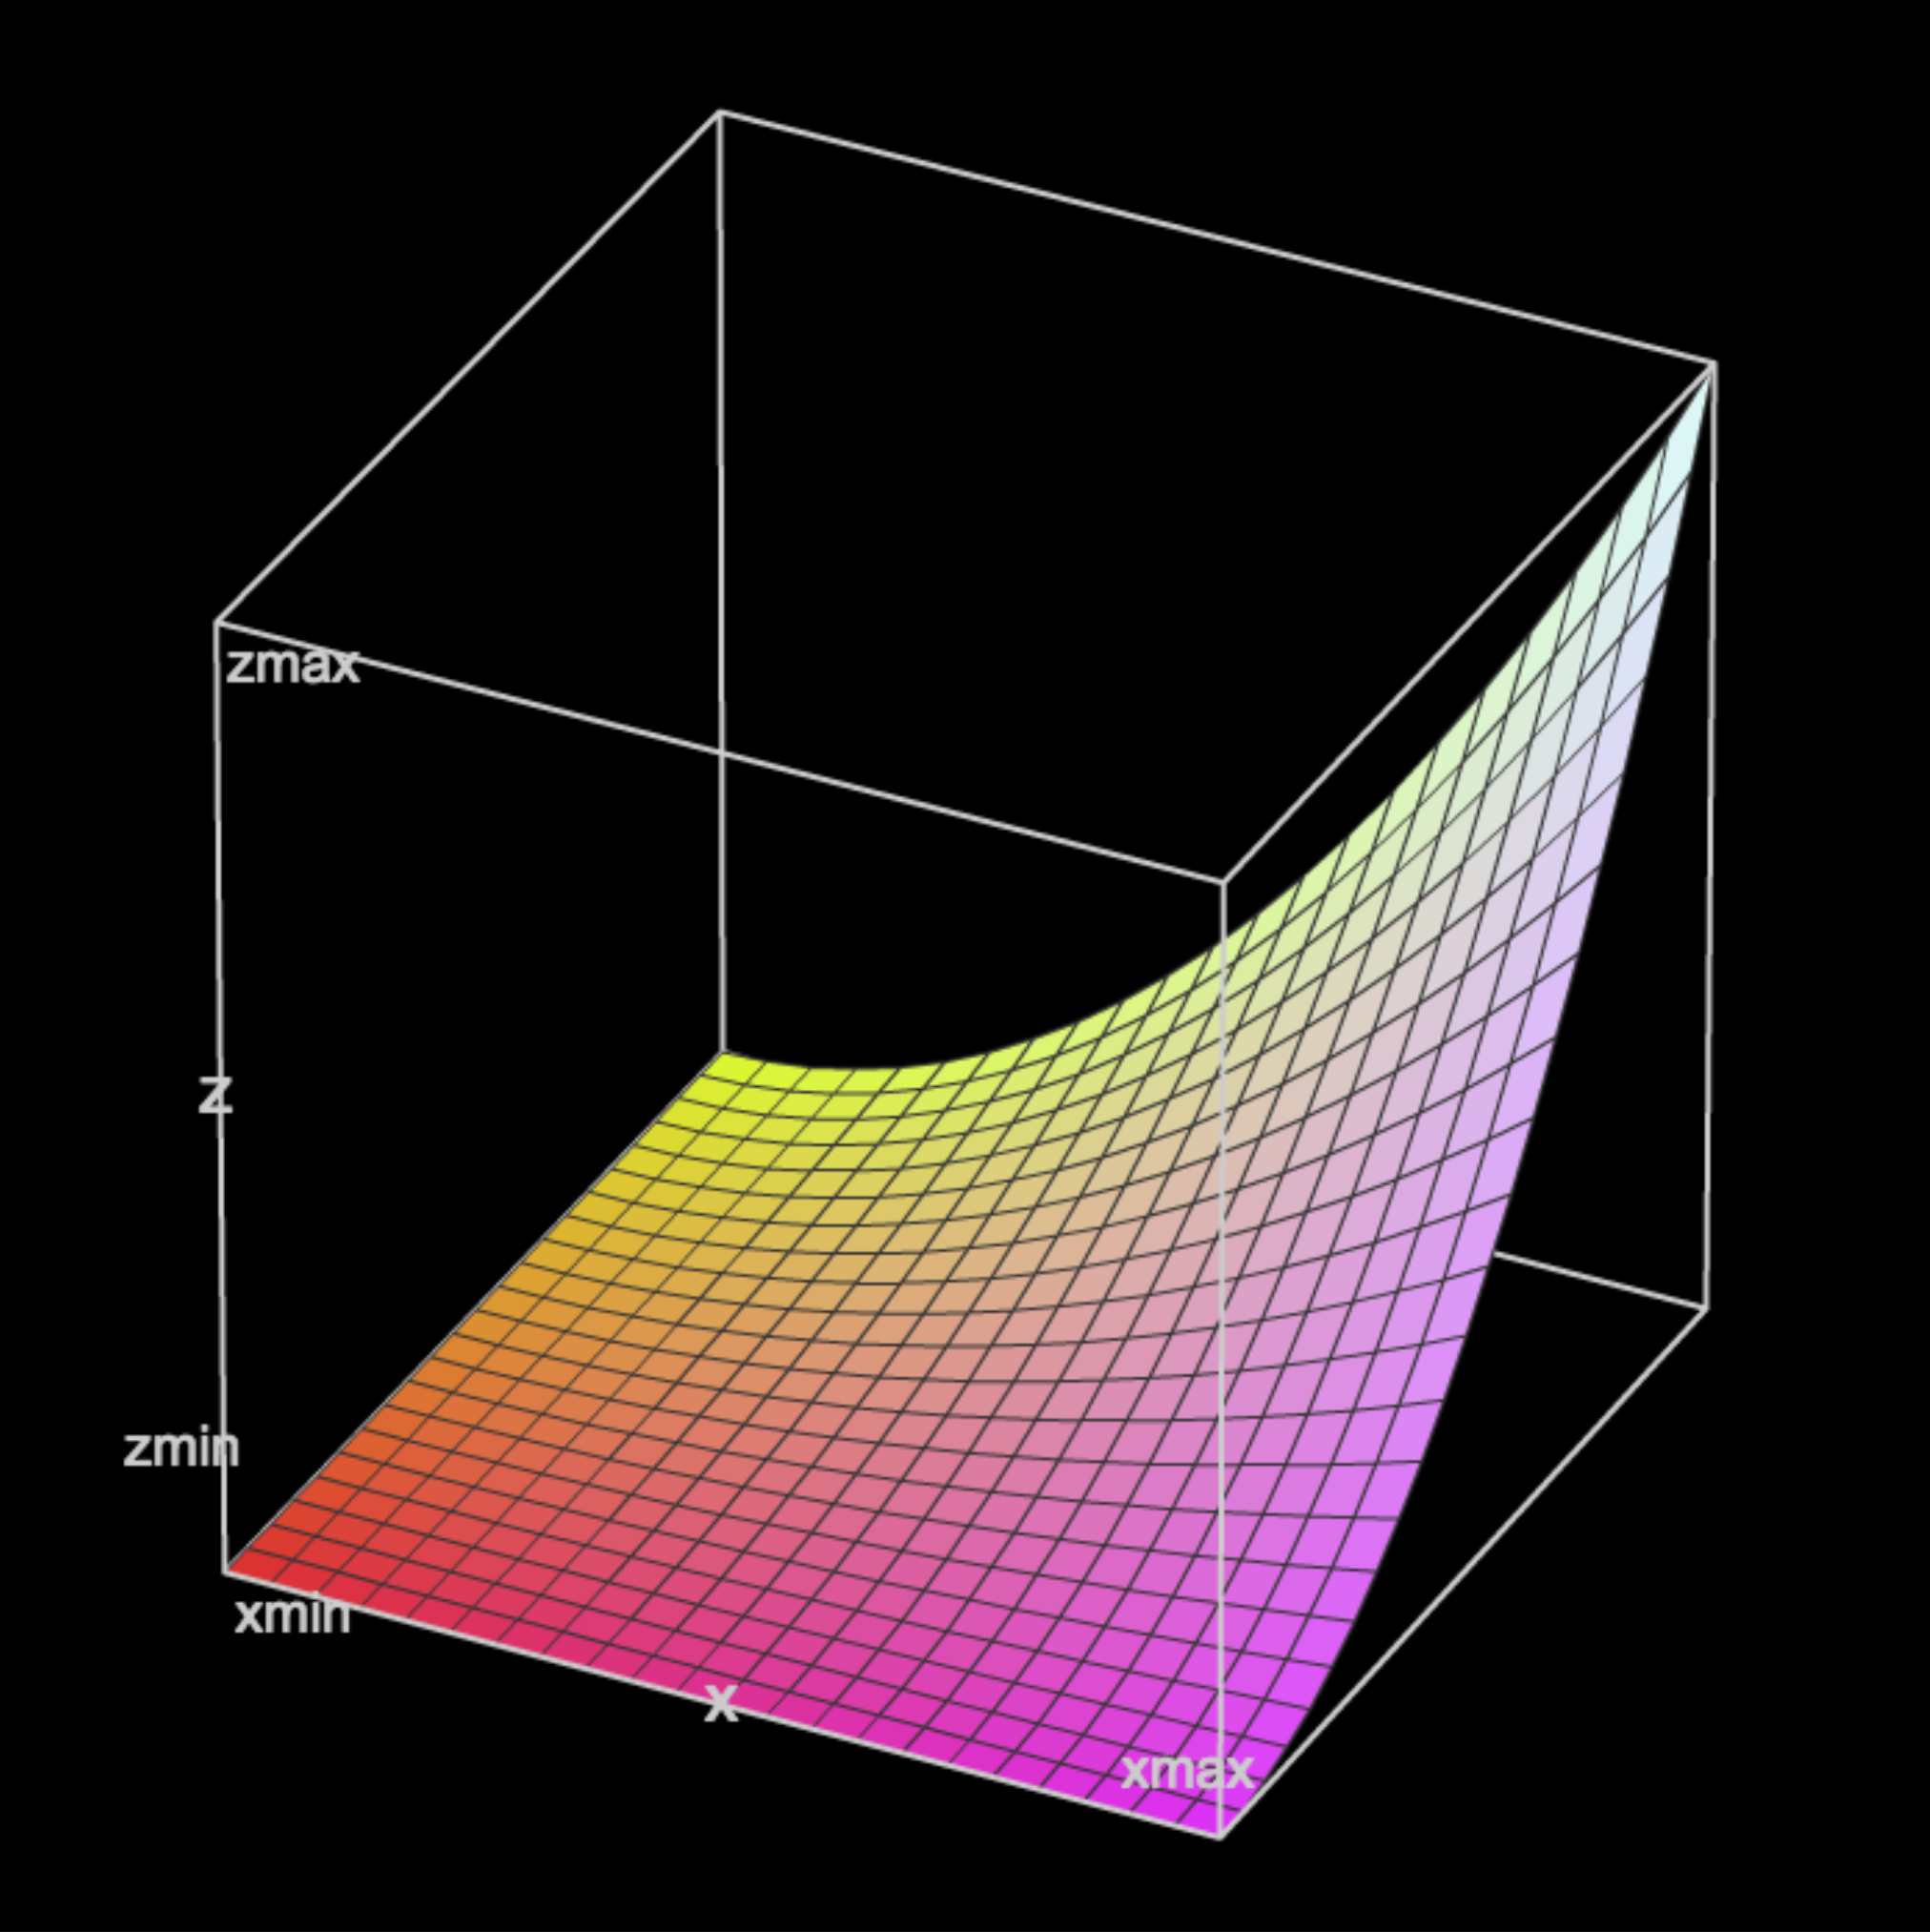
\includegraphics[width=\linewidth]{squared-3b}
	\caption{Cuadrática, ecuación~\ref{eq:sqr}}
	\label{fig:squared3}
\end{figure}

\begin{figure}[p]
	\centering
	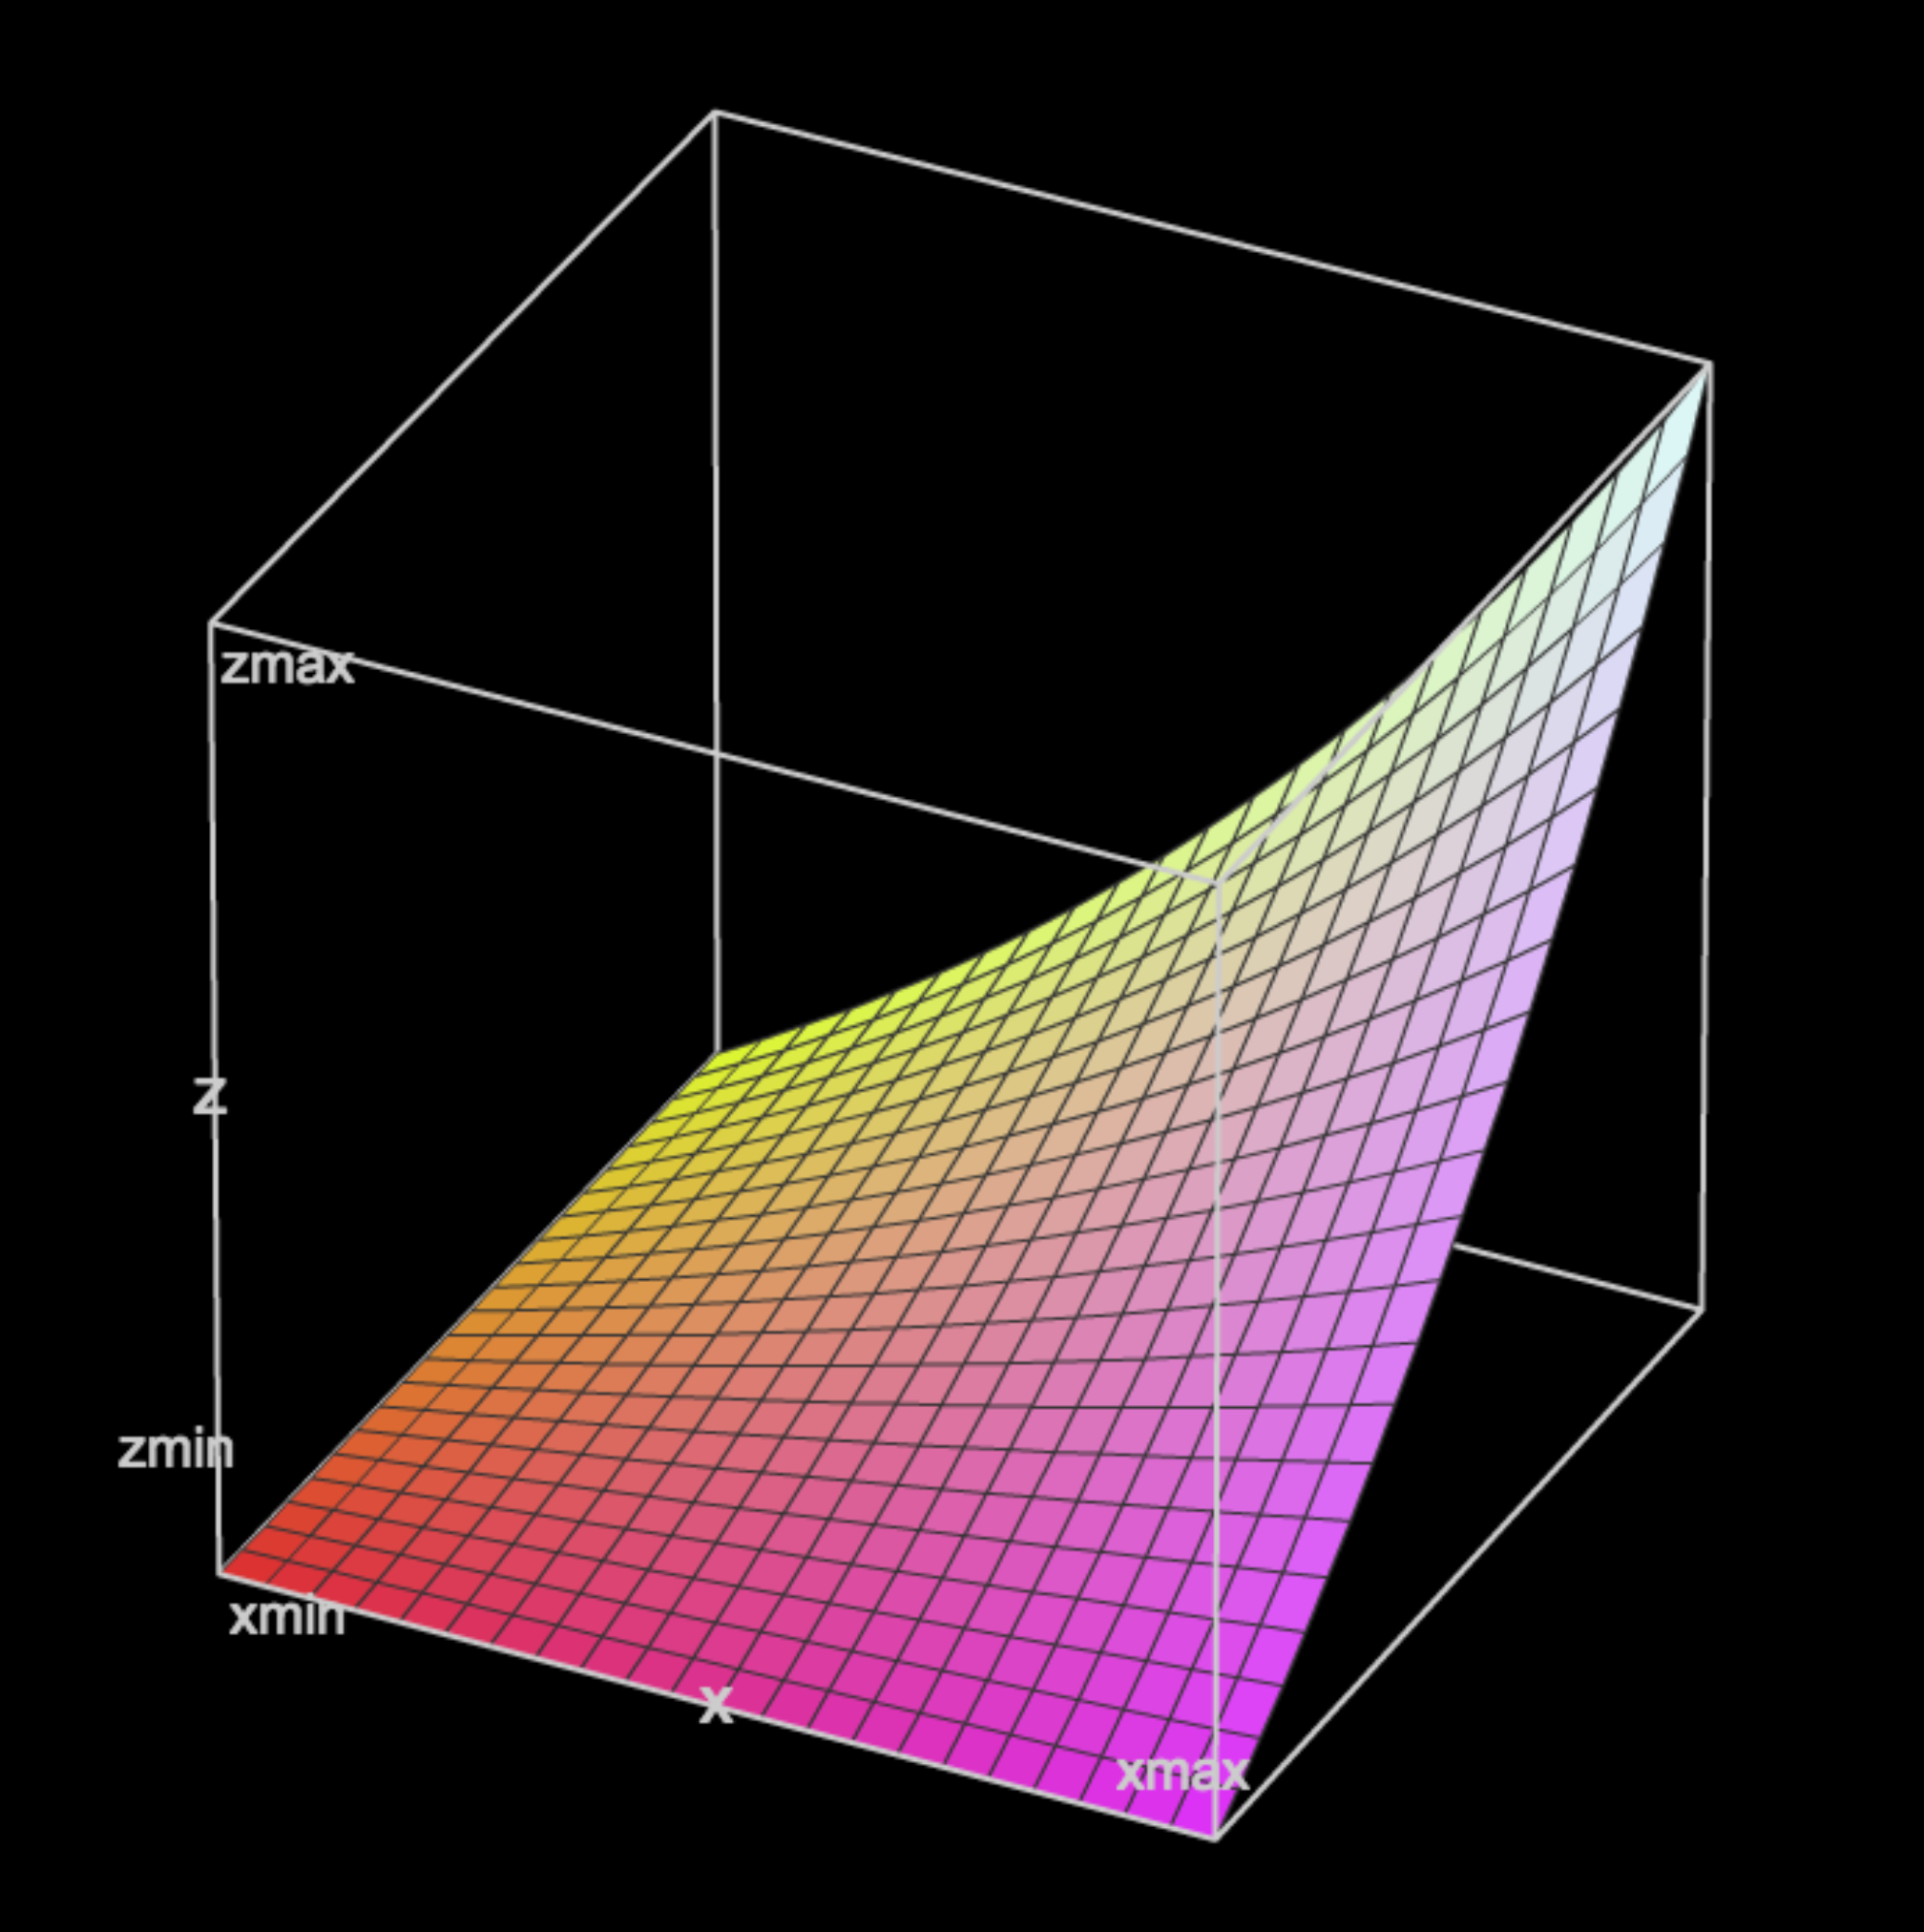
\includegraphics[width=\linewidth]{euler-3b}
	\caption{Euler, ecuación~\ref{eq:exp}}
	\label{fig:euler3}
\end{figure}

\subsection{Resultados}


XXX INSERTAR RESULTADOS XXX
\section*{Conclusiones}

Aquí concluyen.

%---------------------------- Bibliography -------------------------------

% Please add the contents of the .bbl file that you generate,  or add bibitem entries manually if you like.
% The entries should be in alphabetical order
\small
\bibliographystyle{abbrv}

\begin{thebibliography}{99}

\bibitem{pgnn2002}
G. Toussaint
\newblock Proximity Graphs for Nearest Neighbor Decision Rules: Recent Progress.
\newblock {\em Interface}, vol 34, 2005.

\bibitem{evo2003}
CANO, José Ramón; HERRERA, Francisco; LOZANO, Manuel.
\newblock Using evolutionary algorithms as instance selection for data reduction in KDD: an experimental study.
\newblock {\em Evolutionary Computation, IEEE Transactions on}, vol. 7, no 6, p. 561-575., 2003.

\bibitem{psfnn2012}
Garcia, S., Derrac, J., Cano, J. R., \& Herrera, F.
\newblock Prototype selection for nearest neighbor classification: Taxonomy and empirical study
\newblock {\em  Pattern Analysis and Machine Intelligence, IEEE Transactions on}, 34(3), 417-435, 2012

\end{thebibliography}


% \newpage
% \section*{Apéndice}

\end{document}
